\documentclass[journal,10pt,twocolumn]{article}
\usepackage{graphicx}
\usepackage[margin=0.5in]{geometry}
\usepackage[cmex10]{amsmath}
\usepackage{array}
\usepackage{booktabs}
\title{\textbf{Line Assignment}}
\author{Hari Venkateswarlu}
\date{September 2022}
\usepackage[framemethod=tikz]{mdframed}
\newcommand{\myvec}[1]{\ensuremath{\begin{pmatrix}#1\end{pmatrix}}}
\let\vec\mathbf
\newcommand{\mydet}[1]{\ensuremath{\begin{vmatrix}#1\end{vmatrix}}}
\providecommand{\mbf}{\mathbf}
\providecommand{\pr}[1]{\ensuremath{\Pr\left(#1\right)}}
\providecommand{\qfunc}[1]{\ensuremath{Q\left(#1\right)}}
\providecommand{\sbrak}[1]{\ensuremath{{}\left[#1\right]}}
\providecommand{\lsbrak}[1]{\ensuremath{{}\left[#1\right.}}
\providecommand{\rsbrak}[1]{\ensuremath{{}\left.#1\right]}}
\providecommand{\brak}[1]{\ensuremath{\left(#1\right)}}
\providecommand{\lbrak}[1]{\ensuremath{\left(#1\right.}}
\providecommand{\rbrak}[1]{\ensuremath{\left.#1\right)}}
\providecommand{\cbrak}[1]{\ensuremath{\left\{#1\right\}}}
\providecommand{\lcbrak}[1]{\ensuremath{\left\{#1\right.}}
\providecommand{\rcbrak}[1]{\ensuremath{\left.#1\right\}}}

\begin{document}

\maketitle
\paragraph{\textit{Problem Statement} - Find a point on the x-axis,which is equidistant from the points$\begin{pmatrix}
  7 \\
  6 \\
 \end{pmatrix}$ and $\begin{pmatrix}
  3 \\
  4 \\
 \end{pmatrix}$}
\begin{enumerate}
\item finding the point on x-axis which is equidistant from the points
\end{enumerate}

\begin{figure}[h]
\centering
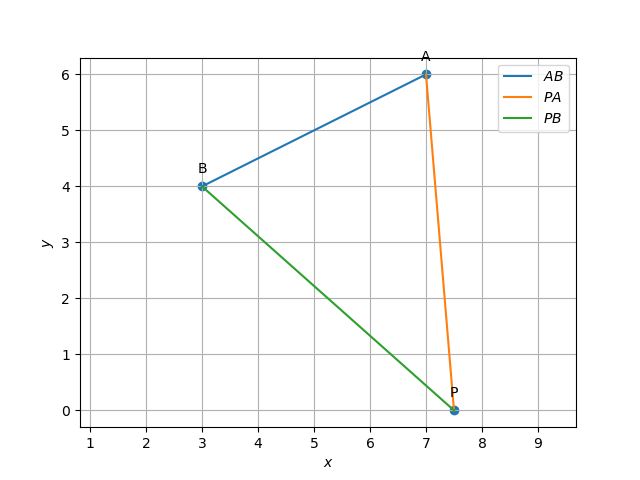
\includegraphics[width=1\columnwidth]{Figure1.png}

\label{fig}
\end{figure}

\section*{Solution}
1. Given points
A=$\begin{pmatrix}
  7 \\
  6 \\
 \end{pmatrix}$
 and B=$\begin{pmatrix}
  3 \\
  4 \\
 \end{pmatrix}$


\raggedright 2. If the point is lying on x-axis then y-axis will be zero i.e.. y=0


\raggedright 3. Distance between the points  $\begin{pmatrix}
  7 \\
  6 \\
 \end{pmatrix}$ and $\begin{pmatrix}
  x \\
  0 \\
 \end{pmatrix}$ is equal to distance between the points $\begin{pmatrix}
  3 \\
  4 \\
 \end{pmatrix}$ and $\begin{pmatrix}
  x \\
  0 \\
 \end{pmatrix}$\\ 	     

\raggedright 4. Consider P on x-axis P$\begin{pmatrix}
  x \\
  0 \\
 \end{pmatrix}$           \vspace{3mm}
\begin{align}
	||\vec{A-P}|| = ||\vec{B-P}||
\end{align}  
    $||\vec{A-P}|| = \vec{\sqrt{{(A-P)}^{\top}{(A-P)}}}$\\
    
$ \vec{\|A-P\|} = \sqrt{\myvec{7-x\\6}\myvec{7-x & 6}}$ \\
$ \vec{\|A-P\|} = (7-x)^2+36$ \\
    $||\vec{B-P}|| =  \vec{\sqrt{{(B-P)}^{\top}{(B-P)}}}$\\   
    $||\vec{B-P}|| = \sqrt{\myvec{3-x\\4}\myvec{3-x & 4}}$\\
    $||\vec{B-P}|| = (3-x)^2+16$ \\
    \vspace{1mm}
 \raggedright 5. From equation 1 
 \\
    \vspace{1mm}            
\begin{gather*}
 (7-x)^2+36=(3-x)^2+16\\                      
 (7-x)^2+20=(3-x)^2\\                         
 49+x^2-14x+20=9+x^2-6x\\                     
 60=8x\\                                    
 x=60/8\\                               
 x=7.5   
\end{gather*}               			
\end{document}
